\input{../article_base.tex}
\title{פתרון מטלה 06 --- משוואות דיפרנציאליות, 80320}
% chktex-file 9
% chktex-file 17

\usepackage{pgfplots, tikz, pgffor}
\usetikzlibrary{math}
\pgfplotsset{compat=1.18}

\begin{document}
\maketitle
\maketitleprint[blue]{}

\question{}
\subquestion{}
נגדיר,
\[
	A
	= \begin{pmatrix}
		-5 & 1 \\
		4 & -2
	\end{pmatrix}
.\]
נמצא פתרון כללי למשוואה $x'(t) = A x(t)$ ונצייר דיאגרמות זרימה מתאימה.
נקבע אם הראשית היא נקודת שיווי משקל יציבה או לא.
\begin{solution}
	נגדיר $P_A(t) = \det(I t - A) = (t + 5)(t + 2) - 4 = (t + 6)(t + 1)$ פולינום אופייני ולכן $A$ לכסינה וכן $A = P^{-1} \diag(-6, -1) P$ לאיזושהי $P \in M_2(\RR)$ הפיכה.
	נחשב את $P$ על־ידי מציאת וקטורים עצמיים,
	\[
		(A + 6 I) u = 0
		\iff \begin{pmatrix}
			1 & 1 \\
			4 & 4
		\end{pmatrix} u = 0
		\iff u = \Sp\{ {(1, -1)}^t \}
	.\]
	וכן,
	\[
		(A + I) u = 0
		\iff \begin{pmatrix}
			-4 & 1 \\
			4 & -1
		\end{pmatrix} u = 0
		\iff u = \Sp\{ {(1, 4)}^t \}
	.\]
	כלומר אם נגדיר,
	\[
		P
		= \begin{pmatrix}
			1 & 1 \\
			-1 & 4
		\end{pmatrix}
	.\]
	היא מטריצה הפיכה המלכסנת את $A$.
	ממשפט פתרון משוואות לינאריות נסיק שהפונקציה,
	\[
		x(t)
		= P^{-1} e^{\diag(-6, -1) t} P x_0
		= P^{-1} \diag(e^{-6 t}, e^{-t}) P x_0
	.\]
	הוא הפתרון היחיד למשוואה $x'(t) = A x(t), x(0) = x_0$.

	נשרטט את הזרימה:
	\begin{otherlanguage}{english}
		\begin{center}
			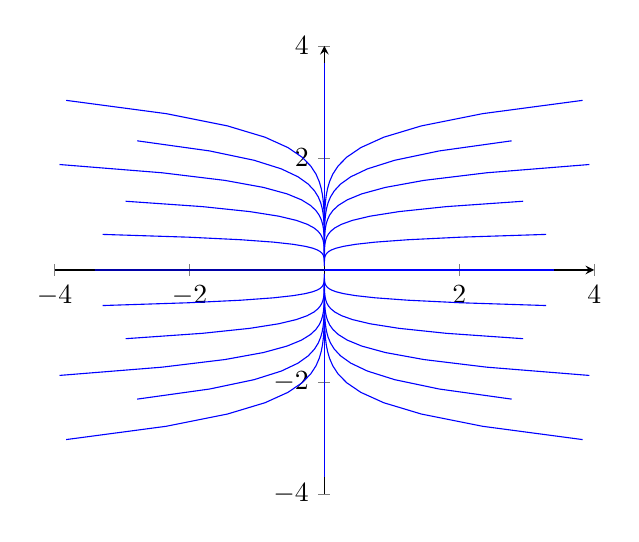
\begin{tikzpicture}
				\begin{axis}[ymin=-4,
						ymax=4,
						xmin=-4,
						xmax=4,
						samples=50,
						axis y line=middle,
						axis x line=middle,
						restrict x to domain=-4:4,
						restrict y to domain=-4:4,
						clip=true]
					\foreach \k in {0,1,...,23} {
						\edef\X{cos(360 * \k / 24)}
						\edef\Y{2 * sin(360 * \k / 24)}
						\addplot [blue,domain=-2:2,samples=50,variable=\t] ({exp(-6 * \t) * \X}, {exp(-1 * \t) * \Y});
					}
				\end{axis}
			\end{tikzpicture}
		\end{center}
	\end{otherlanguage}
	כאשר $x$ מתרחק מ־$0$ בזמן חיובי ומתקרב ל־$0$ בזמן שלילי. \\
	בהתאם נסיק ש־$0$ אכן נקודת שיווי משקל לא יציבה בזמן חיובי ויציבה בזמן שלילי.
\end{solution}

\subquestion{}
נמיר את המשוואה $x'' + x' - 2x = 0$ במערכת משוואות מסדר ראשון, נמצא פתרון ונצייר דיאגרמה.
\begin{solution}
	אנו יודעים כי ניתן להמיר על־ידי המטריצה,
	\[
		A = \begin{pmatrix}
			0 & 1 \\
			2 & -1
		\end{pmatrix}
	.\]
	הפעם נקבל,
	\[
		P_A(t)
		= t (t + 1) - 2
		= t^2 + t - 2
		= (t - 1)(t + 2)
	.\]
	לנוחות הקורא נדלג על חישוב הווקטורים העצמיים ונכריז שעבור,
	\[
		P = \begin{pmatrix}
			1 & 1 \\
			1 & -2
		\end{pmatrix}
	.\]
	מקיימת $A = P^{-1} \diag(1, -2) P$.
	אז נקבל שהפתרון של $y'(t) = A y(t), y(0) = y_0$ הוא,
	\[
		y(t)
		= P^{-1} \diag(e^t, e^{-2t}) P y_0
	.\]
	נשרטט את הפתרון ל־$y$ אשר שקול ל־$x$,
	\begin{otherlanguage}{english}
		\begin{center}
			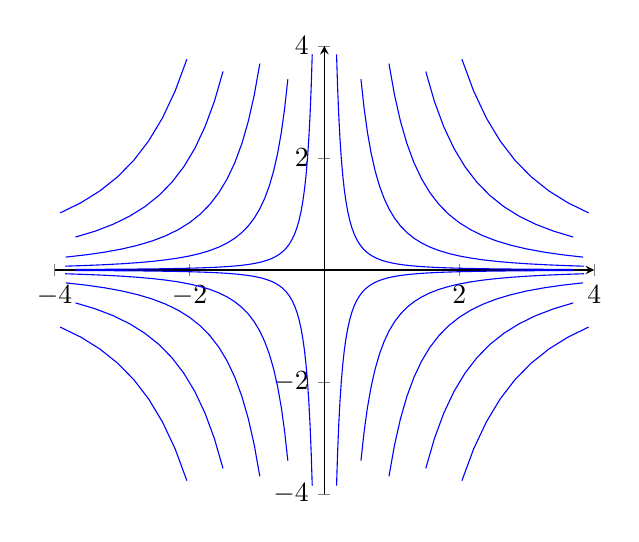
\begin{tikzpicture}
				\begin{axis}[ymin=-4,
						ymax=4,
						xmin=-4,
						xmax=4,
						samples=50,
						axis y line=middle,
						axis x line=middle,
						restrict x to domain=-4:4,
						restrict y to domain=-4:4,
						clip=true]
					\foreach \k in {-5,-4,...,5} {
						\edef\X{\k/2}
						\addplot [blue,domain=-2:2,samples=50,variable=\t] ({exp(\t) * \X}, {exp(-2 * \t) * \X});
						\addplot [blue,domain=-2:2,samples=50,variable=\t] ({exp(\t) * \X}, {exp(-2 * \t) * (-\X)});
					}
				\end{axis}
			\end{tikzpicture}
		\end{center}
	\end{otherlanguage}
	והפעם נקבל ש־$0$ לא נקודת שיווי משקל באף כיוון.
\end{solution}

\question{}
תהי $F : \Omega \to \RR^n$ ליפשיץ מקומית ונגדיר את בעיית תנאי ההתחלה,
\[
	\begin{cases}
		x'(t) = F(x(t)) \\
		x(0) = x_0
	\end{cases}
	\tag{1}
.\]
נניח כי כל הקורדינטות של $F$ אי־שליליות.
תהי $U \subseteq \Omega$ כך שגם $\bar{U} \subseteq \Omega$ ונסמן את הפתרון המקסימלי של $(1)$ ב־$x$.
נראה כי אחת מהאפשרויות הבאה מתקיימת:
\begin{enumerate}
	\item $x$ מגיע לשפה של $U$ בזמן סופי
	\item $\lim_{t \to \infty} x(t) \in \bar{U}$ ונקודה זו היא נקודת שיווי משקל של $F$
\end{enumerate}
\begin{proof}

\end{proof}

\end{document}
